\documentclass[pdflatex,sn-mathphys-num]{sn-jnl}

% --- math / physics ---
\usepackage{amsmath,amssymb}
\usepackage{physics}
\usepackage{bm}
% --- figures / floats ---
\usepackage{graphicx}
\usepackage{float}
\usepackage{subcaption}
% --- algorithms ---
\usepackage{algorithm}
\usepackage{algpseudocode}
\usepackage{xcolor}
% --- revision markup: \rev{...} highlights newly inserted/edited text in red. ---
% Save the REAL \textcolor BEFORE neutralizing author draft colors, so that
% \rev stays coloured even though plain \textcolor{...}{...} is stripped below.
\let\origtextcolor\textcolor
\definecolor{revred}{RGB}{200,30,30}
\newcommand{\rev}[1]{{\origtextcolor{revred}{#1}}}
% --- neutralize draft working-note colors (\textcolor{c}{txt} -> txt) ---
\renewcommand{\textcolor}[2]{#2}

% custom double-ket used in the Liouville-space notation
\newcommand{\ketket}[1]{\left| #1 \right\rangle \! \mathclose{\left. \vphantom{#1} \right\rangle}}

% Springer template sets this (sn-article.tex): prevents vertical glue from being
% stretched to fill sparse pages, which otherwise blows up spacing around displays.
\raggedbottom

\begin{document}

\title[Quantum Mpemba Effect]{Quantum Mpemba Effect in Disordered Lattices}

\author[1]{\fnm{P.\,E.} \sur{Chuklanov}}
\author[1]{\fnm{M.\,A.} \sur{Less}}
\author[2]{\fnm{P.\,V.} \sur{Zakharenko}}
\author[1]{\fnm{D.\,E.} \sur{Zaitsev}}
\author*[2]{\fnm{A.\,P.} \sur{Alodjants}}\email{Alexander\_ap@list.ru}

\affil[1]{\orgname{Moscow Institute of Physics and Technology}, \orgaddress{\city{Dolgoprudny}, \country{Russia}}}
\affil[2]{\orgname{ITMO University}, \orgaddress{\city{Saint Petersburg}, \country{Russia}}}

\abstract{We investigate the Quantum Mpemba effect (QME) in which a quantum state initially farther from equilibrium relaxes faster than one starting closer. We consider single-photon dynamics in networks of coupled optical waveguides to examine QME. The system is modeled as a quantum walk on a graph subject to local dephasing within the Lindblad master equation framework. By spectrally decomposing the Liouvillian superoperator for regular square lattices, we identify initial states with selective mode content that exhibit pronounced anomalous relaxation. We then introduce a Watts--Strogatz-type edge-rewiring procedure and show that topological disorder enhances the population-sector localization of the slowest relaxation sector more strongly than that of the next slow modes. Motivated by this localization contrast, we directly calculate local-excitability maps and identify ``bright'' and ``dark'' regions with respect to the fundamental mode, enabling a spectrally informed spatial construction of Mpemba state pairs. Based on this finding, we propose a deterministic heuristic algorithm that generates initial states with a pronounced Mpemba effect for selected disordered lattice topologies and validate it against Monte Carlo sampling.}

\keywords{Quantum Mpemba effect, Disordered lattices, Open quantum systems, Quantum walks}

\maketitle

\section{Introduction} 
%The Mpemba effect---the counter-intuitive observation that a system initially \emph{further} from equilibrium can relax to its stationary state \emph{faster} than one starting closer---has fascinated scientists since antiquity and was systematically documented by Mpemba and Osborne in 1969 for the case of hot water freezing faster than cold~\cite{Mpemba1969}. Despite half a century of debate in classical thermodynamics, the origin and generality of the effect remained elusive until a modern theoretical framework rooted in spectral analysis of relaxation dynamics was developed.  A key insight is that anomalous relaxation occurs when the initial state has a suppressed overlap with the slowest decaying eigenmode of the generator governing the dynamics, so that faster-decaying channels dominate the approach to equilibrium.  In the classical domain, this picture was confirmed experimentally in colloidal systems, where exponentially accelerated cooling was demonstrated in a controlled setting~\cite{Kumar2020}.

The Mpemba effect is a counterintuitive relaxation phenomenon in which a system initially farther from equilibrium reaches its stationary state faster than one that starts closer. It was first systematically described by Mpemba and Osborne in 1969 for hot water freezing faster than cold~\cite{Mpemba1969}. Subsequent studies revealed that this effect is not limited to thermal systems but can be understood more generally through the spectral structure of relaxation dynamics --- a framework established for Markovian systems by Lu and Raz~\cite{Lu2017} and sharpened by the strong-Mpemba classification of Klich~\emph{et al.}~\cite{Klich2019}. Within this framework, anomalously fast relaxation occurs when the initial state has a weak overlap with the slowest decaying eigenmode of the dynamical generator; the relaxation is then governed primarily by faster modes, and the system approaches equilibrium more quickly. This mechanism has been confirmed experimentally in classical colloidal systems, where accelerated cooling was observed under controlled conditions~\cite{Kumar2020}.

In quantum physics, the Mpemba effect acquires a richer structure (see~\cite{AresReview2025} for a recent review). Transplanting the classical spectral mechanism~\cite{Lu2017,Klich2019} to the quantum domain, Carollo,
Lasanta, and Lesanovsky~\cite{Carollo2021} showed that in Markovian open quantum systems governed by a Lindblad master equation,
an appropriately engineered unitary rotation of the initial state can render it orthogonal to the slowest Liouvillian eigenmode, thereby
\emph{exponentially} accelerating the approach to stationarity. This strong form of the QME relies on the spectral decomposition of
the Liouvillian superoperator: if the overlap coefficient $c_1$ with the first non-trivial right eigenvector vanishes, the effective
relaxation gap is set by the second eigenvalue and convergence becomes exponentially faster. In~\cite{Kochsiek2022}, the authors subsequently demonstrated that global spin rotations can serve as a practical, albeit approximate, implementation of this idea in dissipative spin lattices, providing a physically realizable protocol for accelerated relaxation.
 
The QME has since been predicted and observed across a wide range of physical platforms.
In isolated many-body quantum systems, an analogous effect manifests
through anomalous symmetry restoration: a tilted ferromagnet with
\emph{greater} initial symmetry breaking can restore its symmetry
\emph{faster} than one closer to the symmetric state, as probed
via entanglement asymmetry~\cite{Ares2023}.
The  experimental observation of this phenomenon was reported by Joshi~\emph{et al.}~\cite{Joshi2024} using a trapped-ion quantum simulator, where the effect was monitored through randomized measurements and classical shadows.
In the domain of open quantum systems, the strong QME---characterized
by an exponentially accelerated approach to the steady state---was
experimentally demonstrated in~\cite{Zhang2025} on a single trapped-ion qubit.
In that work, the strong Mpemba condition was shown to coincide with a Liouvillian exceptional point,
revealing a deep connection between anomalous relaxation and non-Hermitian physics. The thermodynamic content of the effect has likewise been analyzed in mesoscopic transport settings~\cite{Chatterjee2023} and through the lens of work and entropy production~\cite{Moroder2024}. Photonic lattices provide a particularly natural and experimentally
accessible arena for studying the QME. In particular, Longhi~\cite{Longhi2024} demonstrated that the Mpemba effect arises
in the diffusive dynamics of light in finite-sized photonic lattices under dephasing: certain highly localized initial intensity
distributions reach the uniform (equilibrium) distribution faster than initially delocalized ones.  
%An experimentally feasible realization based on optical pulse propagation in  temporal mesh lattices was proposed in the same work.
Extending these results to the genuinely quantum-optical regime,
Longhi~\cite{Longhi2024bosonic} predicted a \emph{bosonic} Mpemba
effect in leaky optical resonators and waveguides by exploiting
non-classical states of light---Fock states, coherent states, and
squeezed states---whose distinct photon statistics lead to
qualitatively different relaxation pathways.
Together, these photonic studies establish coupled waveguide networks
as a versatile and tunable platform for engineering anomalous
relaxation phenomena, bridging the gap between abstract spectral
theory and concrete quantum-optical implementations. 

\rev{The models studied here sit at the interface between anomalous relaxation and quantum transport on complex networks. Continuous-time quantum walks provide a natural framework for coherent transport on graphs of arbitrary topology~\cite{Mulken2011}, and the interplay between such coherent dynamics and dephasing underlies the phenomenon of dephasing-assisted transport, in which a controlled amount of decoherence can enhance rather than suppress excitation transfer~\cite{Plenio2008}. A property of network spectra that is central to the present study is the localization of Laplacian (and, more generally, generator) eigenvectors on heterogeneous graphs: slow relaxation modes tend to concentrate on subsets of nodes with characteristic degree, so that topology alone can render a mode spatially localized~\cite{Hata2017}. We show below that the same mechanism operates for the dephasing Liouvillian and provides the geometric handle we exploit to engineer Mpemba state pairs.}

In this work, we investigate the QME on graphs that model networks of coupled optical waveguides. We consider the
quantum walk of a single photon with local dephasing described by a Lindblad master equation. The
central idea is to exploit the spatial structure of the Liouvillian
eigenmodes---specifically, the distinction between ``bright'' modes
(efficiently excited by local perturbations) and ``dark'' modes
(spatially decoupled from most of the network)---to engineer initial
states with controlled overlap with the slowest relaxation channels.
The role of network topology, and in particular the transition from
regular to disordered lattices via an edge-rewiring
procedure, is a key element of our analysis.


The paper is organized as follows.
In Sec.~2, we introduce the model: the tight-binding Hamiltonian
for single-photon walks on graphs, the Lindblad master equation
with local dephasing dissipators, and the distance metric based on
quantum relative entropy used to identify the Mpemba effect.
In Sec.~3, we present the Liouvillian vectorization and spectral
decomposition formalism.
In Sec.~4, we analyze the mode structure of regular square lattices,
constructing spatial population maps and identifying geometric
regularities.
In Sec.~5, we use the spectral decomposition to design candidate
initial states with selective mode content and verify the Mpemba
effect through numerical simulation.
In Sec.~6, we describe the Watts--Strogatz-type edge-rewiring
procedure that interpolates between regular and random topologies,
and characterize the associated rewiring-induced path-length crossover.
In Sec.~7, we perform a detailed spectral and eigenvector analysis
of the disordered lattices, tracking the evolution of relaxation rates,
the Inverse Participation Ratio, and the community overlap of the
slowest modes as functions of the rewiring probability. We identify
topology-induced population-sector localization of the slow mode and examine
the mode-resolved spatial concentration of local excitability.
In Sec.~8, we leverage the local excitability maps to propose a
deterministic heuristic algorithm for constructing pairs of initial
states that exhibit a pronounced Mpemba effect on selected network
topologies, and validate it against Monte Carlo sampling.
Finally, Sec.~9 summarizes the main results and discusses perspectives
for future work.
 

%\textcolor{blue}{In this study, we examine fundamental models of quantum system dynamics in networks of coupled optical waveguides. The structure of this work follows a progression from regular to disordered systems.} 


%\textcolor{blue}{First, we treat the waveguide system as a graph and construct the model for photon dynamics. We narrow our focus to regular lattices, for which we analytically derive the explicit form of the corresponding Lindbladians. By investigating the mode structure in these systems, we construct the first examples of initial states that demonstrate the Mpemba effect. Next, using a rewiring procedure, we transition from regular lattices to random graphs and observe how the mode behavior evolves. To explain the observed spectral changes, we introduce hypotheses concerning localization and differences between "dark" and "bright" modes. We then use this "dark/bright" framework to construct excitability (illumination) maps for the graphs. Finally, based on these maps, we propose an algorithm that constructs the initial state with the most pronounced Mpemba effect for any given topology.}



\section{Model}

\subsection{Hamiltonian of Single-Photon Walk on a Graph}
Let us consider the quantum walk of a single photon in a network of coupled optical waveguides~\cite{tang2018}. In such arrays the role of time is played by the propagation distance along the waveguides, so all temporal dynamics below translates directly into evolution along the sample~\cite{tang2018,Longhi2024}. In the tight-binding approximation, the dynamics of the system are governed by the Hamiltonian:
\begin{equation}
\hat{H} = -\frac{J}{2}\sum_{i,j} \tau_{ij}(\hat{a}_i^{\dagger}\hat{a}_j + \hat{a}_j^{\dagger}\hat{a}_i),
\end{equation}
where $\hat{a}_i^\dagger$ ($\hat{a}_i$) is the photon creation (annihilation) operator at site $i$, $J$ is the connection constant (hopping rate), which is the same for all nodes, and $\tau$ is the symmetric adjacency matrix of the $N$-node graph.

To include environmental decoherence into our model, we employ the Lindblad master equation framework~\cite{lindblad1976,gks1976,breuer2002}. For a network of optical waveguides, the dominant source of decoherence is local dephasing, which is described by the local number operators acting as dissipators, $\hat{L}_k = \hat{a}_k^\dagger \hat{a}_k = \hat{n}_k$. Coherent hopping supplemented by local dephasing places the model in the class of quantum stochastic walks, which interpolate between coherent quantum and classical diffusive transport~\cite{Whitfield2010}. Physically, pure dephasing captures the random propagation-constant fluctuations induced by fabrication disorder and environmental noise, which destroy inter-site phase coherence while conserving the photon number; this is the dominant decoherence channel considered in photonic realizations of anomalous relaxation~\cite{Longhi2024}. Uniform propagation losses --- the other ubiquitous imperfection --- factor out of the single-photon sector as a global attenuation and leave the \emph{normalized} relaxation dynamics, and hence all trajectory crossings studied below, unchanged; site-resolved loss engineering is beyond the scope of this work. The evolution of the system's density matrix $\hat{\rho}$ is given by:
\begin{equation}
\frac{d\hat{\rho}}{dt} = -i[\hat{H}, \hat{\rho}] + \gamma \sum_{k=1}^N \left( \hat{L}_k \hat{\rho} \hat{L}_k^\dagger - \frac{1}{2}\{\hat{L}_k^\dagger \hat{L}_k, \hat{\rho}\} \right),
\end{equation}
where $\gamma > 0$ is the dephasing rate. 

We consider the dynamics strictly within the single-photon subspace, spanned by the localized basis states $|k\rangle$. In this basis, the number operator acts as a projector, $\hat{n}_k|m\rangle = \delta_{k,m}|m\rangle$. Evaluating the matrix elements $\rho_{k,l} = \langle k|\hat{\rho}|l\rangle$, the coherent part naturally yields $H_{k,m} = -J\tau_{k,m}$ (considering that the adjacency matrix is symmetric due to the non-directionality of the graph). The dissipative part simplifies significantly since $\langle k| \hat{n}_m \hat{\rho} \hat{n}_m |l\rangle = \delta_{k,m}\delta_{l,m}\rho_{k,l}$. Summing over all sites $m$, the full evolution equation reduces to the explicit element-wise form \cite{Longhi2024}:
\begin{equation}
\frac{d\rho_{k,l}}{dt} = iJ \sum_{m=1}^{N} (\tau_{k,m}\rho_{m,l} - \rho_{k,m}\tau_{m,l}) - \gamma(1-\delta_{k,l})\rho_{k,l}.
\label{eq:lindblad_elements}
\end{equation}
As Eq.~(\ref{eq:lindblad_elements}) demonstrates, the dissipative term causes the off-diagonal coherences ($\rho_{k,l}$ for $k \neq l$) to decay at rate $\gamma$, while the diagonal populations ($\rho_{k,k}$) remain unchanged in the absence of hopping.

\subsection{Distance Metric and the Mpemba Effect}
The essence of the Quantum Mpemba effect lies in anomalous relaxation dynamics: a state initially further from equilibrium reaches it faster than a state initially closer. To quantify this phenomenon, we adopt a rigorous geometric distance between the state $\hat{\rho}(t)$ and the stationary state $\hat{\rho}^{(S)}$.

{
Following standard information-theoretic approaches to open quantum systems, we measure the distance to \textcolor{green}{equilibrium using the quantum relative entropy}:
\begin{equation}
D(\hat{\rho}(t) || \hat{\rho}^{(S)}) = \operatorname{Tr}\{\hat{\rho}(t) \log \hat{\rho}(t)\} - \operatorname{Tr}\{\hat{\rho}(t) \log \hat{\rho}^{(S)}\}.
\end{equation}
We choose the quantum relative entropy because it is a fundamental measure of distinguishability between quantum states and is \textcolor{green}{monotonically non-increasing} under completely positive trace-preserving (CPTP) maps \cite{vedral2002}. \textcolor{green}{It represents the quantum generalization of the classical Kullback-Leibler divergence.} While the choice of metric is not uniquely restricted, previous studies indicate that the Quantum Mpemba Effect is a robust dynamical feature qualitatively observable with alternative measures, such as the trace distance or the Hilbert-Schmidt distance \cite{Carollo2021}.

For our model, the stationary state is the maximally mixed state within the single-photon subspace, corresponding to a uniform probability distribution across all $N$ graph nodes: $\hat{\rho}^{(S)} = \frac{1}{N} \hat{I}$. Given that $\operatorname{Tr}(\hat{\rho}) = 1$, substituting this into the relative entropy definition conveniently simplifies the expression to:
\begin{equation}
D(\rho(t)) = \log(N) + \operatorname{Tr}\{\hat{\rho}(t) \log \hat{\rho}(t)\}.
\label{eq:metric}
\end{equation}
Here, the second term is the negative von Neumann entropy of the state~\cite{neumann}. Thus, for the dynamics considered here, the relative entropy and the von Neumann entropy-based distance are mathematically equivalent up to a constant shift. An intersection of the $D(\rho(t))$ trajectories for two distinct initial states $A$ and $B$---that is, $D_A(0) > D_B(0)$ but $D_A(t) < D_B(t)$ at some later time $t>0$---serves as the unambiguous hallmark of the Mpemba effect.
}
\subsection{Liouvillian Vectorization}
To solve Eq.~(\ref{eq:lindblad_elements}) and analyze the system's spectrum, we transition to the Liouville superoperator formalism~\cite{gyamfi2020}. The density matrix is mapped to a column vector via the vectorization operation $\operatorname{vec}(\cdot)$, denoted in double-ket notation as $\ketket{\rho} \equiv \operatorname{vec}(\rho) = [\rho_{1,1}, \rho_{2,1}, \dots, \rho_{N,N}]^\top$. \textcolor{green}{We further define the inverse operator $\operatorname{Mat} \equiv \operatorname{vec}^{-1}$, which restores an $N \times N$ matrix from its vectorized form.} The Liouville space is equipped with the Hilbert-Schmidt inner product $\langle\langle A | B \rangle\rangle = \operatorname{Tr}(A^\dagger B)$.

The master equation transforms into a matrix differential equation $\frac{d}{dt}\ketket{\rho} = L\ketket{\rho}$, where the matrix representation $L$ of the Liouvillian superoperator $\mathcal{L}$ is generally non-normal, $LL^{\dagger}\ne L^{\dagger}L$, and has dimensions $N^2 \times N^2$. It can be explicitly constructed by using the Kronecker product ($\otimes$). Separating the coherent and dissipative parts, we obtain the target matrix:
\begin{equation}
L = iJ(I \otimes \tau - \tau \otimes I) + L_D,
\label{eq:L}
\end{equation}
where $I$ is the $N \times N$ identity matrix, and $L_D$ is a diagonal matrix with elements equal to $0$ for components corresponding to populations ($\rho_{k,k}$) and $-\gamma$ for coherences ($\rho_{k,l}$).\

Throughout the subsequent numerical analysis, we define the time scale in units of the inverse hopping rate, effectively setting \textbf{$J=\frac{1}{2}$} (all times below are quoted in these dimensionless units; in a waveguide implementation they correspond to propagation distance measured in units of the inverse coupling constant). The dephasing rate is fixed at \textbf{$\gamma=0.1$}. This specific ratio ($\gamma/J = 0.2$) places the system in a weakly dissipative regime where coherent dynamics remains appreciable on the relaxation time scale.


\section{Eigenstate Decomposition}
As established, the dynamics equation is written as $\frac{d}{dt}\ketket{\rho} = L \ketket{\rho}$.\\
This implies that its solution can be represented as:
\begin{equation}
\ketket{\rho(t)}=e^{Lt}\cdot \ketket{\rho(0)}
\label{eq:solv_format}
\end{equation}
We analyze the system in the {non-Hermitian} diagonal basis of the operator $L$.\footnote{We assume that the Liouvillian superoperator $L$ is diagonalizable, which guarantees the existence of a complete biorthogonal basis of eigenmodes. While the non-Hermitian nature of $L$ allows for the existence of non-diagonalizable defective degeneracies (Exceptional Points), such points typically form a manifold of measure zero in the parameter space and are avoided in our generic parameter regime. Within an exactly degenerate eigenspace, a numerical eigensolver returns a linearly independent basis whose particular choice is not unique.} This vectorization formalism allows for the spectral analysis of the Liouvillian superoperator.\cite{minganti2018}

To spectrally decompose the dynamics, we introduce a biorthogonal basis consisting of the right eigenvectors $v_k \ (\ketket{\rho_k})$ and the left eigenvectors $\langle\langle\sigma_k |$, which satisfy:
\begin{equation}
L\cdot v_k = \lambda_k \cdot v_k,
\quad
\langle\langle \sigma_j | \rho_k\rangle\rangle = \mathcal{N}_k \delta_{jk},
\label{eq:eig_1}
\end{equation}

\textcolor{green}{Throughout, the right eigenvectors are normalized as $\lVert v_k\rVert_2=1$. The quantity $\mathcal{N}_k$ is a complex normalization constant. While analytical treatments often set $\mathcal{N}_k = 1$, standard numerical eigensolvers normalize left and right eigenvectors independently. Therefore, we explicitly retain the factor $\mathcal{N}_k = \langle\langle\sigma_k | \rho_k\rangle\rangle$ in all subsequent projections.}
\begin{equation}
\ketket{\rho(0)}=\sum_k c_k v_k
\label{eq:eig_decomp_0}
\end{equation}
Substituting this decomposition into the dynamics formula yields:
\begin{equation}
\ketket{\rho(t)}=\sum_kc_ke^{\lambda_k t }v_k
\label{eq:eig_decomp}
\end{equation}

{We uniquely identify the stationary state of the system corresponding to $\lambda_0=0$. The associated right eigenvector is the stationary density matrix $v_0 = \ketket{\rho^{(S)}}$, and the corresponding left eigenvector is the identity operator. Due to the trace-preserving nature of the Lindblad evolution, the coefficient for the stationary mode is strictly $c_0 = 1$, since $\langle\langle\sigma_0|\rho\rangle\rangle = \operatorname{Tr}\rho = 1$ both for the initial and for the stationary state. }


Furthermore, $e^{\operatorname{Re}\lambda_k t}$ represents the dissipative exponent in the decomposition; thus, $\operatorname{Re}\lambda_k < 0$ for non-trivial modes, corresponding to the decay rate. The term $e^{i\operatorname{Im}\lambda_k t}$ corresponds to the oscillation frequency $\omega_k = \operatorname{Im}\lambda_k$. \cite{kessler2012, minganti2018}

\section{Lattice Investigation}
Let us begin the analysis with a small \textbf{square} lattice.\

To this end, we construct mode population maps. The mode $k$, corresponding to the eigenvector $v_k$, is reshaped into matrix form via the $\operatorname{Mat}$ operator defined in Sec.~2.3. It is crucial to emphasize that $\operatorname{Mat}(v_k)$ does not represent a physical state: it is not positive semi-definite, and for every non-stationary mode its trace vanishes exactly, $\operatorname{Tr}\operatorname{Mat}(v_k)=\langle\langle\hat{I}|\rho_k\rangle\rangle=0$, since the left eigenvector associated with $\lambda_0=0$ is the identity. Consequently, the diagonal components plotted below sum to zero. Then, the populations (diagonal components) are extracted from the resulting matrix; each such component corresponds to a single lattice site:
\begin{equation}
\vec{p}_k = \operatorname{Re}(\operatorname{diag}(\operatorname{Mat}(v_k))).
\label{eq:p_k}
\end{equation}
The components of $\vec{p_k}$ are then mapped onto the \textbf{nodes of the original lattice}. In the diagram, color and brightness are normalized across the entire plot and illustrate the sign and magnitude, respectively.\\
\textcolor{green}{
Because the ideal square lattice possesses fundamental geometric symmetries (the $D_4$ point group), the Liouvillian superoperator commutes with the corresponding spatial symmetry operators and its spectrum contains symmetry-related exact degeneracies. Here and below, degeneracy means coincidence of the full complex eigenvalue $\lambda$. Distinct complex-conjugate eigenvalues $\lambda$ and $\lambda^*$ share the same $\operatorname{Re}(\lambda)$ and may therefore belong to the same relaxation-rate group, but they are not degenerate unless they coincide; this pairing is not analyzed separately. Within an exactly degenerate eigenspace, the particular basis returned by the numerical eigensolver is not physically unique, so the analysis below uses basis-invariant group quantities such as $W_{k'}$ and $d_i$.}

To systematically present these results without redundancy, the modes are organized into relaxation-rate groups $k'$ sharing identical values of $\operatorname{Re}(\lambda)$. Fig.~\ref{fig:big_modes_map} illustrates a representative basis for a $10 \times 10$ lattice.

\begin{figure}[H]
    \centerline{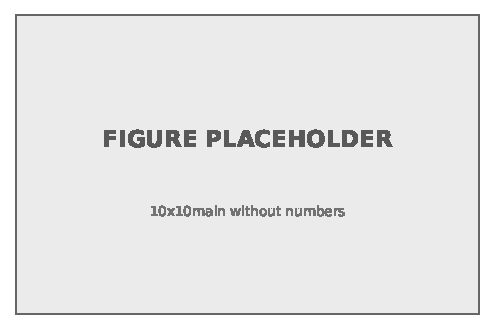
\includegraphics[width=0.9\linewidth]{figures/10x10main_without_numbers}}
    \caption{Node-wise distribution of Liouvillian eigenmode populations for a $10 \times 10$ regular lattice. The maps represent the real part of the diagonal components of the reshaped eigenvectors $\vec{p_k}$ (eq. \ref{eq:p_k}). Modes are organized into relaxation-rate groups $k'$ sharing identical values of $\operatorname{Re}(\lambda)$; for example, the group $k'=1$ contains modes $k=1, \dots, 4$. Color intensity of each node is normalized globally by the maximum absolute population value, $\max |p_k|$, found among all non-trivial modes. Red denotes positive values, blue indicates negative values, with opaque colors corresponding to a relative amplitude of $\pm 1$ (i.e., $\pm 100\%$ of $\max |p_k|$).}
    \label{fig:big_modes_map}
\end{figure}


\section{Analysis of Mode Structure}


Analysing the spatial mode distributions, we find distinct geometric regularities, as exemplified by the $10 \times 10$ lattice in Fig.~\ref{fig:big_modes_map}. Rather than resembling random noise, the slow modes exhibit clear, macroscopic patterns governed by lattice symmetries. Examining the figure, we immediately observe that the modes in the slowest relaxation-rate group ($k'=1$) are strongly localized at the lattice boundaries and corners. As the decay rate increases, these macroscopic features shift, giving rise to pronounced diagonal and anti-diagonal structural motifs (e.g., $k'=2$ and $k'=21$). Conversely, as the mode index increases further, the spatial distributions become less globally expressive. The higher-order modes lose their macroscopic structure, breaking down into fine-grained, small-scale spatial fluctuations (high spatial frequencies) that eventually resemble unstructured noise.

This clear structural hierarchy---from macroscopic, boundary-localized patterns to fine-scale local fluctuations---provides a powerful heuristic principle for investigating the Quantum Mpemba effect.\footnote{As defined in Sec.~2.2, the Quantum Mpemba effect occurs when a state with a larger initial distance $D(\rho(0))$ relaxes to the stationary state faster than one with a smaller initial distance, leading to a crossing in their distance trajectories.} Initial states engineered to geometrically match the macroscopic "footprint" of specific slow modes are highly likely to excite those modes with extreme selectivity. Guided by this physical insight, we construct a set of eight distinct candidate initial states. These states serve as our "candidates" for demonstrating anomalous relaxation, as they are explicitly designed to couple predominantly into only a handful of targeted relaxation channels.

The empirical candidate states for a square lattice are defined as follows:\\
\begin{enumerate}
    \item \textbf{Pure (Center):} A photon localized at a single central site (for even $n$, any of the four central sites), probing modes with central density.
    \item \textbf{Mixed (Two Corners):} An equal mixture of states at two opposite corners, \textit{targeting the symmetries seen in $k'=1, 4, 5, 7, 22$ in Fig.~\ref{fig:big_modes_map}.}
    \item \textbf{Mixed (Four Corners):} A statistical mixture of all four corner sites.
    \item \textbf{Mixed (Diagonal):} An incoherent mixture of sites along the main diagonal, \textit{subspaces like $k'=2, 21$ in Fig.~\ref{fig:big_modes_map}.}
    \item \textbf{Pure (Coherent Diagonal):} A coherent superposition supported entirely on the geometric main diagonal: $|\psi\rangle = \frac{1}{\sqrt{|S|}}\sum_{j\in S}|j\rangle$ with $S = \{(i, j) : i = j\}$.
    \item \textbf{Mixed (Inner Corners):} A mixture of the four inner corners $\{(2, 2), (n-1, 2), (2, n-1), (n-1, n-1)\}$.
    \item \textbf{Mixed (Top/Bottom Edges):} A state distributed evenly along the top and bottom boundary rows. \textit{E.g. $k'=2,3,4,7$ in Fig.~\ref{fig:big_modes_map}}
    \item \textbf{Mixed (Checkerboard):} A macroscopic checkerboard pattern (e.g., only "even" nodes occupied), \textit{specifically designed to interact with high-frequency modes similar to $k'=26$ in Fig.~\ref{fig:big_modes_map}.}

\end{enumerate}




To verify our heuristic selection, we quantitatively evaluate the magnitude of the mode contribution to each state by computing the projection onto the corresponding Liouvillian eigenbasis:
\begin{equation}
c_k = \frac{\langle\langle\sigma_k | \rho(0) - \rho^{(S)}\rangle\rangle}{\langle\langle\sigma_k | \rho_k\rangle\rangle}
\label{eq:c_k}
\end{equation}

Where: $ \ketket{\rho(0)}$ --- vectorized initial density matrix. $\ketket{\rho^{(S)}}$ --- vectorized stationary state density matrix. $\ketket{\rho_k}$ --- $k$-th right eigenvector of the Liouvillian ($v_k$). $\langle\langle\sigma_k | $ --- $k$-th left eigenvector of the Liouvillian ($w_k^\dagger$).\textcolor{green}{ The pairwise normalization by $\langle\langle\sigma_k | \rho_k\rangle\rangle$ is well defined only when the full complex eigenvalue is non-degenerate. Within exactly degenerate eigenspaces of the regular lattice the numerically returned left and right eigenvectors are not necessarily biorthogonally paired, so in practice the coefficients are obtained as the exact solution of the linear system $\sum_k c_k \ketket{\rho_k} = \ketket{\rho(0) - \rho^{(S)}}$; the accuracy of every decomposition is monitored through its reconstruction residual ($\leq 10^{-10}$ for all eight states).}

In the right diagram (Fig.~\ref{fig:candidate_states}), we plot the percentage contribution of each relaxation-rate group $k'$, $W_{k'} = \|\sum_{k \in k'} c_k \ketket{\rho_k}\|^2$, normalized over the non-stationary groups. Within an exactly degenerate eigenspace, individual coefficients $c_k$ depend on the arbitrary basis choice made by the numerical eigensolver, whereas the norm of the projected component is basis-invariant. {The weights $W_{k'}$ do not possess a direct probabilistic interpretation. Instead, they serve as a relative geometric measure of how strongly a specific transient channel is excited by the initial configuration.}



We decompose each of the 8 candidate initial states into the lattice eigenbasis to quantify their mode content. The projection coefficients $W_k$ indicate how strongly a specific mode participates in the relaxation process of a given state. The results, summarized in Fig.~\ref{fig:candidate_states}, confirm that our empirically chosen states are indeed highly selective. \textcolor{green}{The bar charts reveal a striking sparsity: the incoherent mixtures couple to a small number of relaxation-rate groups rather than smearing across the spectrum. This is a direct consequence of \textbf{symmetry selection rules}: because these states exhibit distinct spatial symmetries (e.g., the fully symmetric "Four Corners"), their overlaps vanish for eigenmodes of mismatched spatial parity. The coherent superposition (state 5), which also populates the off-diagonal coherence sectors, couples to a broader yet still structured set of groups.} This symmetry-driven selectivity is the fundamental prerequisite for observing the trajectory crossings characteristic of the Quantum Mpemba effect.

\begin{figure}[H]
    \centerline{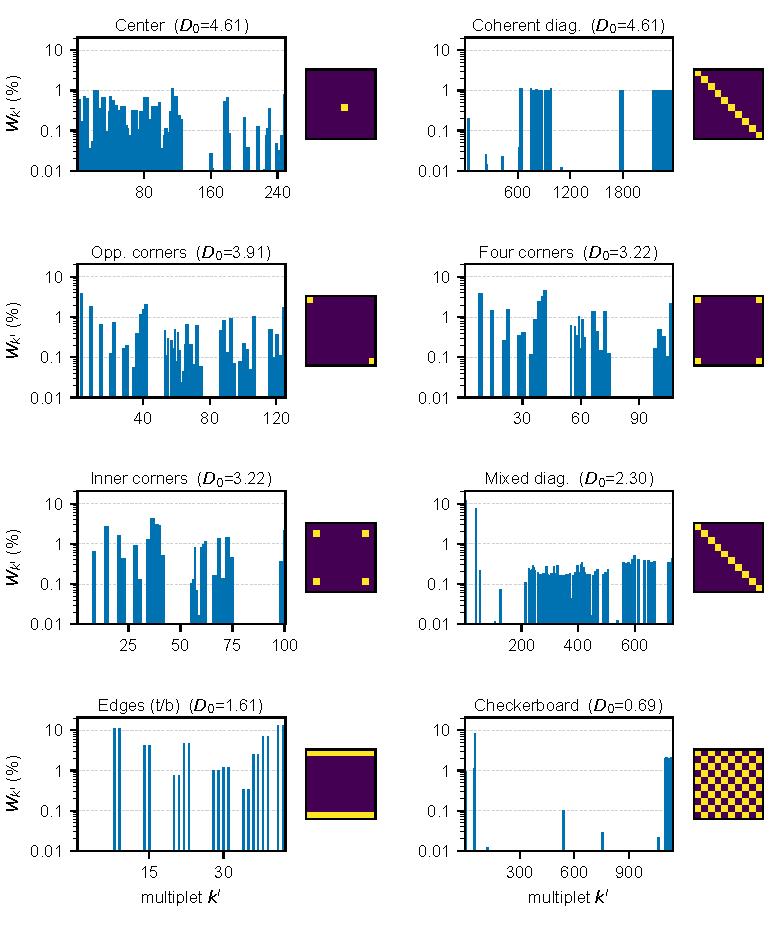
\includegraphics[width=1.0\linewidth]{figures/new_tabled_10x10_bar_chart_log_ENG_new_8STATES}}
    \caption{Spectral decomposition of eight candidate initial states in a $10 \times 10$ lattice. Each \textbf{panel} analyzes a specific initial condition and consists of two elements: (1) a bar chart of the relaxation-rate-group weights $W_{k'}$ --- the squared norm of the state's component within each group $k'$ (cf. eq. \ref{eq:c_k}) --- plotted on a \textbf{logarithmic scale} (left); and (2) a schematic illustration of the initial photon distribution (right), where yellow cells indicate nodes with a non-zero initial photon probability, serving as a binary visual guide independent of exact statistical weights or quantum phases. Panels are ordered by decreasing initial distance to equilibrium $D_0=D(\rho(0))$.}
    \label{fig:candidate_states}
\end{figure}
To avoid a misleadingly sparse appearance in linear scale (where the dominant bar masks the remaining weights), we present only the logarithmic visualization. The log scale highlights the intended point: the selected initial states have a strongly \emph{mode-selective} decomposition while still exhibiting nonzero projections onto multiple faster modes.\

\subsection{Simulation}
We then perform a time-evolution simulation for these states to verify the predicted effect. As shown in Fig.~\ref{fig:simulation_lattice_10x10}, the trajectories for specific pairs cross, confirming the phenomenon. This behavior is robust and has been observed across a range of square lattice sizes ($n\in\{5,\dots,11\}$).


\begin{figure}[H]
    \centerline{
\includegraphics[width=1\linewidth]{figures/9states_modes_simulation_line_10x10_with_selection_ENG}}
    \caption{Relaxation dynamics of the $10\times 10$ lattice system shown as the time evolution of the distance to equilibrium $D(\rho(t))$ for eight distinct initial states (see Fig.~\ref{fig:candidate_states}). The crossing of trajectories (bold) represents the Mpemba effect, which is observed for the state pair (2 and 5).}
    \label{fig:simulation_lattice_10x10}
\end{figure}

\textcolor{green}{\section{Network Rewiring}}
We now perturb the lattice structure by randomly rewiring a fraction of the edges. This process involves switching edge endpoints, thereby conserving the total number of edges in the system. The topology is governed by the parameter $p \in [0, 1]$, representing the rewiring probability for each initial edge. For an open $n \times n$ square lattice, the exact number of undirected edges is $E = 2n(n-1)$. The expected number of attempted rewiring events is therefore $Ep=2n(n-1)p$, while the realized mean satisfies $\langle E_{\mathrm{rew}} \rangle \approx 2n(n-1)p$ and differs slightly because events without a valid target are bypassed and the ensemble is conditioned on connectivity.

In the context of open quantum systems, network fragmentation produces multiple degenerate stationary states---mirroring the classical correspondence between the multiplicity of the graph-Laplacian zero eigenvalue and the number of connected components~\cite{fiedler1973}---which makes the stationary state non-unique, so that the long-time limit depends on the initial condition and the single relaxation gap relative to one equilibrium state loses its meaning. Therefore, we must strictly enforce the global connectivity of the network. We achieve this through a Monte Carlo rejection sampling procedure, detailed in Algorithm~\ref{alg:rewiring}.

\begin{algorithm}[H]
\caption{Connectivity-Guaranteed Edge Rewiring}
\label{alg:rewiring}
\begin{algorithmic}[1]
\Require Lattice dimension $n$, rewiring probability $p$, optional PRNG $seed$
\Ensure Connected adjacency matrix $\tau$
\State Initialize pseudo-random number generator with $seed$ (if provided)
\State $connected \gets \mathbf{false}$
\While{not $connected$}
    \State $\tau \gets \text{generate\_base\_grid}(n \times n)$
    \State $\mathcal{E} \gets \text{list of all edges in } \tau$; Randomly shuffle $\mathcal{E}$
    \For{each edge $(u, v) \in \mathcal{E}$}
        \If{$\operatorname{rand}(0, 1) < p$}
            \State Select node $X$ uniformly from $\{u, v\}$
            \State Let $Y$ be the other node: $Y \gets \{u, v\} \setminus \{X\}$
            \State $\mathcal{V}_{\text{valid}} \gets \text{all nodes} \setminus (\{X, Y\} \cup \text{neighbors of } X \text{ in } \tau)$
            \If{$\mathcal{V}_{\text{valid}} \neq \emptyset$}
                \State Select target $W$ uniformly from $\mathcal{V}_{\text{valid}}$
                \State Remove edge $(X, Y)$ and add edge $(X, W)$ to $\tau$
            \EndIf
        \EndIf
    \EndFor
    \If{$\text{check\_connectivity\_BFS}(\tau) == \mathbf{true}$}
        \State $connected \gets \mathbf{true}$
    \EndIf
\EndWhile
\State \Return $\tau$
\end{algorithmic}
\end{algorithm}

To prevent the creation of self-loops and multi-edges, target nodes are restricted to the set $\mathcal{V}_{\text{valid}}$. If no valid targets remain for a selected edge, its rewiring is simply bypassed (lines 11--14). Disconnected realizations are discarded via Breadth-First Search (BFS) validation (lines 17--19). This rejection step conditions the statistical ensemble on global connectivity: the acceptance fraction is essentially unity for $p \lesssim 0.05$, decreases to ${\approx}86\%$ at $p=0.3$, and reaches ${\approx}20\%$ at $p=1$, so ensemble averages at strong rewiring refer to the connected subensemble. Finally, to guarantee the exact reproducibility of the representative single-graph spatial maps presented in subsequent sections, the generator is initialized with a fixed seed. For statistical ensemble averaging, the seed varies to ensure independent sampling.

\vspace{1em}
\textit{Unless stated otherwise, the following sections use $10 \times 10$ lattices.}

\subsection{Classical Network Analysis}

A standard method for investigating structural crossovers in networks involves analyzing the average shortest path length (averaged over all node pairs) as a function of the disorder parameter---in our case, the rewiring probability $p$ \cite{barthelemy}. For a more comprehensive analysis of network path-length crossovers and the broader small-world property, see \cite{newman, kleinberg}.

We plot this dependence for a $10 \times 10$ lattice across different scales. To isolate the rewiring-induced path-length crossover~\cite{watts1998} for this specific macroscopic metric, the strict BFS connectivity filter (Algorithm~\ref{alg:rewiring}) was relaxed: graphs were rewired in a single pass without the rejection step, and the average shortest-path length of each realization was computed over its largest connected component (which coincides with the full graph whenever the realization is connected). The goal of this figure is to identify the crossover region in $p$ that will later be compared with spectral changes:
\begin{figure}[H]
\centering
\begin{subfigure}{0.49\linewidth}
    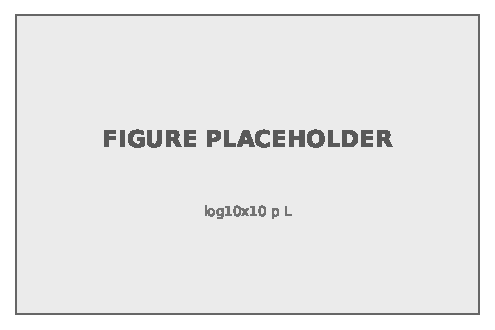
\includegraphics[width=1\linewidth]{figures/log10x10_p_L}
    \caption{full scale}
\end{subfigure}
\hfill
\begin{subfigure}{0.49\linewidth}
    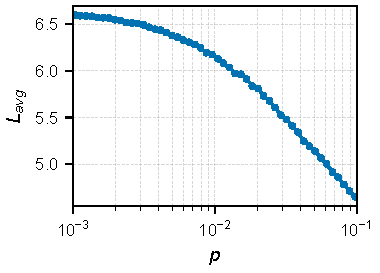
\includegraphics[width=1\linewidth]{figures/log10x10_p_L_SCALED}
    \caption{crossover region}
\end{subfigure}
\caption{Average shortest-path length versus rewiring probability $p$ (in log. scale) for a $10\times 10$ lattice, shown in two scalings. The smooth rewiring-induced path-length crossover identifies the range in which adding long-range links sharply reduces typical graph distances; no separate clustering-based small-world criterion is imposed.}
\label{fig:path_length_crossover}
\end{figure}
We observe a smooth path-length crossover over intermediate rewiring probabilities. The value $p=0.15$ used below is a representative intermediate-disorder working point, not a uniquely defined transition threshold.

\section{Mode Analysis for Disordered Lattices}
We now turn to the analysis of disordered lattices obtained via the rewiring model described above, where the network topology is parameterized by the lattice size and the rewiring probability $p \in [0, 1]$. Our goal  here is to understand how the spectral and spatial properties of the Liouvillian eigenmodes evolve as the network transitions from a regular lattice to a disordered graph.

\subsection{Spectral Analysis}

To establish a baseline for our spectral analysis, Fig.~\ref{fig:rewired_spectra} presents representative Liouvillian eigenvalue spectra across several orders of magnitude of the rewiring probability $p$. This progression illustrates how increasing topological disorder breaks the geometric symmetries of the lattice and modifies the spectral structure near the origin, which governs the long-time relaxation dynamics of the system.




\begin{figure}[H]
\centerline{
\begin{subfigure}{0.32\linewidth}
    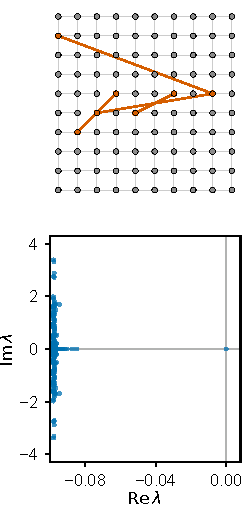
\includegraphics[width=1\linewidth]{figures/with_examples_1}
\end{subfigure}
\begin{subfigure}{0.32\linewidth}
    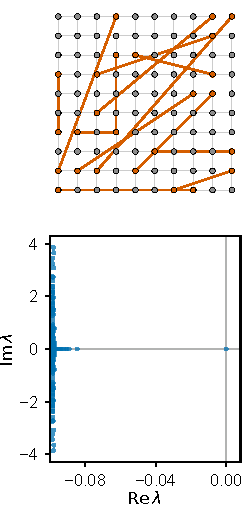
\includegraphics[width=1\linewidth]{figures/with_examples_2}
\end{subfigure}
\begin{subfigure}{0.32\linewidth}
    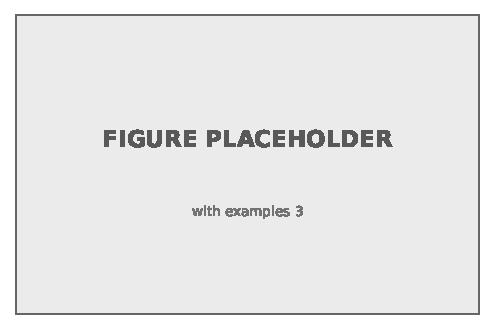
\includegraphics[width=1\linewidth]{figures/with_examples_3}
\end{subfigure}
}
\caption{Representative Liouvillian spectra for rewired $10\times 10$ lattices at increasing disorder levels ($p=0.01$, $p=0.1$, $p=0.3$). At weak disorder ($p=0.01$) the spectrum retains the structured, near-degenerate branches inherited from the lattice symmetry; increasing the rewiring probability lifts these degeneracies and progressively smears the spectral branches. The eigenvalues closest to zero (rightmost points) correspond to the slowest relaxation modes.}
\label{fig:rewired_spectra}
\end{figure}


\subsection{Analysis of Slow Modes}
We find that the first few modes, located closest to zero on the real axis, govern the system's long-term dynamics. Note that while these are conventionally the "slowest" decaying modes, they determine the convergence speed.

To elucidate the system's response to disorder, for every realization we identify the slowest non-trivial mode $\lambda_1$ as the eigenvalue with the largest real part. Depending on the realization, this mode is either purely real or belongs to an oscillating complex-conjugate family ($\operatorname{Im}\lambda_1 \neq 0$) inherited from the relaxation-rate groups of the regular lattice. All statistics are collected over 30 independent graph realizations for each $p$; the resulting relaxation rate is shown in Fig.~\ref{fig:modes_log_scale}(a).\

For a detailed analysis across multiple orders of magnitude of $p$, Fig.~\ref{fig:modes_log_scale} presents the mean relaxation rate of the slowest mode, the fraction of realizations in which this mode oscillates, the oscillation frequency of that subensemble, and the separation $\Delta$ between the two slowest \emph{distinct} relaxation rates.

\begin{figure}[H]
\centering
\begin{subfigure}{0.48\linewidth}
    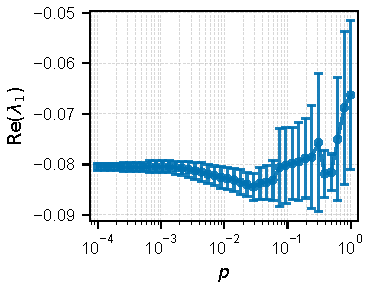
\includegraphics[width=1\linewidth]{figures/re1_p_log}
    \caption{relaxation rate $\operatorname{Re}(\lambda_1)$}
\end{subfigure}
\begin{subfigure}{0.48\linewidth}
    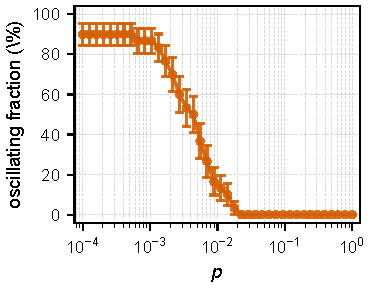
\includegraphics[width=1\linewidth]{figures/oscfrac_p_log}
    \caption{fraction of oscillating realizations}
\end{subfigure}

\vspace{1em}

\begin{subfigure}{0.48\linewidth}
    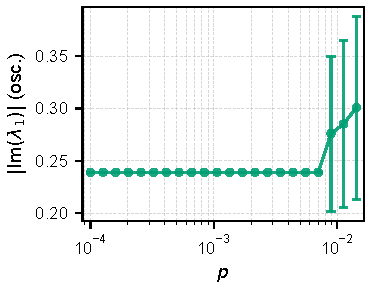
\includegraphics[width=1\linewidth]{figures/im1_p_log}
    \caption{oscillation frequency $|\operatorname{Im}(\lambda_1)|$}
\end{subfigure}
\begin{subfigure}{0.48\linewidth}
    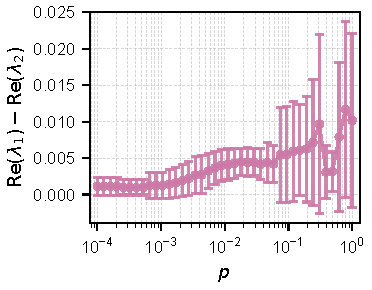
\includegraphics[width=1\linewidth]{figures/sep_p_log}
    \caption{slow-mode separation $\operatorname{Re}(\lambda_1-\lambda_2)$}
\end{subfigure}

\caption{Statistics of the slowest non-trivial Liouvillian mode versus the rewiring probability $p$ (log scale) for a $10 \times 10$ lattice; for each realization the mode is identified by the largest $\operatorname{Re}\,\lambda$. \textbf{(a)} Mean relaxation rate $\operatorname{Re}(\lambda_1)$; the conventional Liouvillian relaxation gap is $-\operatorname{Re}(\lambda_1)$. \textbf{(b)} Fraction of realizations whose slowest mode is oscillating ($\operatorname{Im}\lambda_1 \neq 0$): this fraction falls below one half near $p\approx4\times10^{-3}$, and no oscillating slowest mode is observed in the sampled ensemble for $p\gtrsim2\times10^{-2}$. \textbf{(c)} Mean oscillation frequency $|\operatorname{Im}(\lambda_1)|$ over the oscillating subensemble; points are shown only when at least two oscillating realizations are available. \textbf{(d)} Separation between the two slowest \emph{distinct} relaxation rates, $\Delta = \operatorname{Re}(\lambda_1) - \operatorname{Re}(\lambda_2)$; individual-mode differences are not used when several modes share the same $\operatorname{Re}(\lambda)$. Error bars: $\pm 1$ standard deviation over 30 realizations in (a), (c), (d); binomial standard error in (b).}
\label{fig:modes_log_scale}
\end{figure}
We observe the following. First, at very weak disorder, up to approximately $p=4\times10^{-3}$, the slowest mode is predominantly a member of the oscillating family inherited from the regular lattice ($|\operatorname{Im}\lambda_1| \approx 0.24$). Its fraction then decreases rapidly, and no oscillating slowest mode is observed in the sampled ensemble beyond approximately $2\times10^{-2}$ (panel~b). Second, the mean relaxation rate is \textbf{non-monotonic}: $|\operatorname{Re}(\lambda_1)|$ initially grows with disorder, corresponding to a mild ensemble-averaged \emph{acceleration}, and then decreases toward the random-graph limit, corresponding to a \textbf{slowing down} of the slowest mode. Individual configurations hosting significantly slower localized modes emerge with increasing probability and dominate the ensemble average, which is accompanied by the sharp growth of the realization-to-realization scatter visible in panel~(a).
\textcolor{green}{Rather than constituting the Mpemba effect itself---which strictly refers to the anomalous crossing of relaxation trajectories for specific initial states---this spectral phenomenon represents a \textbf{topology-induced slow-mode localization}. By structurally isolating the slowest relaxation channels, this topological transition geometrically assists in the preparation of initial states that bypass these slow channels, thereby facilitating what we term the \textbf{topologically assisted Quantum Mpemba effect}.}

We confirmed the presence of a similar effect for different dimensions of the square lattice (not shown).




\subsection{Eigenvector Analysis}

To quantify the spatial extent of the eigenmodes, let us consider the Inverse Participation Ratio (IPR)~\cite{farkas},
which characterizes the degree of population-sector localization of the eigenvectors. In the mode matrix $\operatorname{Mat}(v_k)$, we retain only the diagonal components, as we are concerned solely with populations. Throughout this section, ``localization'' therefore refers specifically to localization of this diagonal component; the off-diagonal coherence sector is not included in the IPR or community-overlap measures.
Within an exactly degenerate eigenspace individual eigenvectors are defined only up to a basis rotation, so all localization measures below are evaluated for the distinct relaxation-rate groups $k'$ introduced in Sec.~7.2: the diagonal weight of a group is computed from an orthonormal basis $\{q_k\}$ of the span of its eigenvectors, $d_i = \sum_k |(\operatorname{Mat} q_k)_{ii}|^2$, a quantity invariant under intra-group basis rotations that reduces to $|(\operatorname{Mat} v_k)_{ii}|^2$ for a non-degenerate mode.
We then calculate:
\begin{equation}
IPR(k)=\frac{\sum_{i=1}^N |\rho_{k_{ii}}|^4}{(\sum_{i=1}^N |\rho_{k_{ii}}|^2)^2}
\label{eq:IPR}
\end{equation}
Here, the denominator serves as a normalization factor, ensuring that the IPR value ranges from $1/N$ (for a mode whose diagonal weight is uniformly distributed across all sites) to $1$ (for a mode whose diagonal weight is concentrated at a single site). Consequently, a decrease in this parameter corresponds to a greater delocalization of the mode. To quantitatively trace the structural evolution of the states, we plot the average IPR for the three slowest distinct relaxation-rate groups as a function of the rewiring probability $p$, as shown in Fig.~\ref{fig:ipr_graphs}.

\begin{figure}[H]
\centerline{
\begin{subfigure}{0.32\linewidth}
    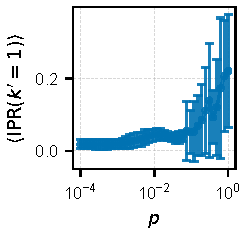
\includegraphics[width=1\linewidth]{figures/10x10_IPR_group_k_1}
    \caption{group $k'=1$}
\end{subfigure}
\begin{subfigure}{0.32\linewidth}
    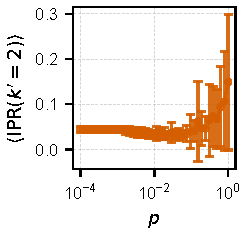
\includegraphics[width=1\linewidth]{figures/10x10_IPR_group_k_2}
    \caption{group $k'=2$}
\end{subfigure}
\begin{subfigure}{0.32\linewidth}
    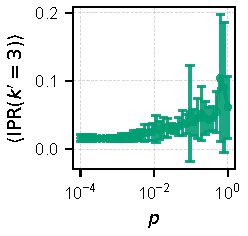
\includegraphics[width=1\linewidth]{figures/10x10_IPR_group_k_3}
    \caption{group $k'=3$}
\end{subfigure}
}
\caption{Dependence of the IPR, defined in Eq.~(\ref{eq:IPR}) with the invariant group weight $d_i$, on the rewiring probability $p$ (log. scale) for the three slowest distinct relaxation-rate groups ($k'=1, 2, 3$) in a $10 \times 10$ lattice. Error bars: $\pm 1$ standard deviation over 30 network realizations. All three groups become more localized with increasing disorder; the leading group shows the strongest growth --- from $\mathrm{IPR} \approx 0.018$ (an extended state inherited from the regular-lattice relaxation-rate group) to $\approx 0.22$ at $p=1$ --- while the subordinate groups localize more weakly.}
\label{fig:ipr_graphs}
\end{figure}
It is worth noting the distinct behavior of the leading group in Fig.~\ref{fig:ipr_graphs}: across the crossover region its IPR exceeds that of the subordinate groups by up to a factor of two, and the steep growth of its localization occurs over the same broad rewiring range as the path-length crossover identified earlier.

\subsection{Community Structure Analysis}
We now establish a complementary, community-based measure of mode localization.
The internal structure of each generated network is identified using the \textbf{Louvain method}, a popular and efficient algorithm \cite{blondel}. It iteratively optimizes the modularity metric by grouping nodes to maximize the density of edges within communities and minimize edges between them. This results in a partition of all $N$ nodes into $N_C$ non-overlapping communities $C_1, C_2, \ldots, C_{N_C}$.

For each Liouvillian eigenmode, we measure its concentration within the identified communities by introducing the \textbf{Overlap coefficient}.
As established previously, the physical meaning of population distribution is carried by the diagonal of the reconstructed mode matrix $\operatorname{Mat}(v_k)$. We define the ``mass'' of the mode at site $i$ as $|\operatorname{Mat}(v_k)_{ii}|^2$.
The total diagonal ``mass'' of the mode, which serves as the normalization denominator in Eq.~(\ref{eq:over_lap}), is:
\begin{equation}
TotalMass(k)=\sum_{i=1}^N|Mat(v_k)_{ii}|^2
\label{eq:total_mass}
\end{equation}

The Overlap of mode $k$ with community $C_m$ is defined as the fraction of its total mass located within that community:
\begin{equation}
Overlap(k, C_m)=\frac{\sum_{i \in C_m}|Mat(v_k)_{ii}|^2}{TotalMass(k)} \ \ \in [0,1]
\label{eq:over_lap}
\end{equation}
\begin{itemize}
    \item If $\max(\operatorname{Overlap}(k)) \approx 1$, the mode is almost entirely contained within a single community. \textbf{It is structurally localized.}
    \item If $\max(\operatorname{Overlap}(k))$ is small (e.g., close to $1/N_C$, where $N_C$ is the number of communities), the mode is distributed across the entire network.
\end{itemize}
To observe the evolution of this structural localization, we calculate the maximum Overlap for the three slowest distinct relaxation-rate groups (using the invariant group weight $d_i$ in place of $|\operatorname{Mat}(v_k)_{ii}|^2$ for exactly degenerate eigenspaces) across different rewiring probabilities $p$. The Louvain partitions are computed with a fixed random seed for reproducibility. The statistically averaged results are presented in Fig.~\ref{fig:community_overlap}.
\begin{figure}[H]
\centerline{
\begin{subfigure}{0.32\linewidth}
    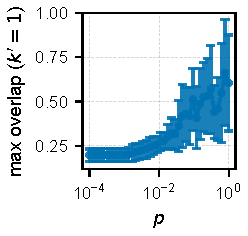
\includegraphics[width=1\linewidth]{figures/10x10_overlap_group_k_1}
    \caption{group $k'=1$}
\end{subfigure}
\begin{subfigure}{0.32\linewidth}
    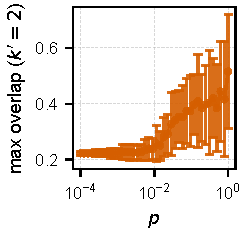
\includegraphics[width=1\linewidth]{figures/10x10_overlap_group_k_2}
    \caption{group $k'=2$}
\end{subfigure}
\begin{subfigure}{0.32\linewidth}
    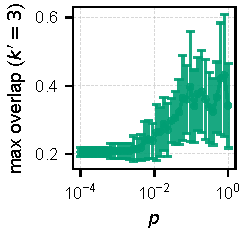
\includegraphics[width=1\linewidth]{figures/10x10_overlap_group_k_3}
    \caption{group $k'=3$}
\end{subfigure}
}
\caption{Dependence of the maximum community Overlap coefficient, defined in Eq.~(\ref{eq:over_lap}), on the rewiring probability $p$ for the three slowest distinct relaxation-rate groups ($k'=1, 2, 3$) in a $10 \times 10$ lattice. Error bars: $\pm 1$ standard deviation over 30 network realizations. The overlap of all three groups grows across the rewiring-induced crossover; the leading group ($k'=1$) reaches the highest confinement (${\approx}0.6$), highlighting its structural localization within specific network communities.}
\label{fig:community_overlap}
\end{figure}

As depicted in Fig.~\ref{fig:community_overlap}, for the regular lattice structure ($p \to 0$), the slow-mode groups are distributed across several symmetry-related regions, and the community overlap is small (${\approx}0.2$). During the crossover, the network locally "breaks down" and connects to distant nodes while retaining local density inherited from the lattice, and the overlap of all three groups grows through the path-length crossover. For the subordinate groups ($k'=2, 3$) the growth is moderate, and only the third group hints at a decline as $p \to 1$, within the realization scatter.\

The leading group, however, stands out, indicating the re-emergence of the previously observed \textbf{topology-induced slow-mode localization}.\\
Its overlap grows monotonically and then reaches a plateau (${\approx}0.6$). Rather than being a strictly quantum anomaly, this behavior represents a fundamental feature of the Liouvillian dynamics in the present dephasing quantum-walk model, sharing structural similarities with the localization of slow relaxation modes in classical diffusion on heterogeneous networks~\rev{\cite{Hata2017,Mulken2011}}. As $p$ increases, particular network regions support increasingly concentrated slow-mode weight, and the modes associated with these regions become the slowest decay channels of the system.

The observed population-sector localization of the slowest mode motivates an examination of its role in the relaxation dynamics. According to the theory of the spectral Mpemba effect, a condition for accelerated relaxation is the ability to prepare an initial state that weakly excites (or "darkens") the slowest mode while strongly interacting with faster modes.\\

For delocalized modes (as in a regular lattice), such "darkening" generally requires interference tuning of amplitudes across the network. In disordered networks, the population-sector concentration of mode $v_1$ motivates a \textbf{spectrally informed spatial construction of excitation}, but it does not by itself determine local excitability because the latter is governed by the left eigenvectors. We therefore \textbf{shift from analyzing the internal right-mode structure to directly calculating the response to local perturbations}.

\subsection{Mode-Resolved State Brightness}
Let us now establish the notion of mode brightness. The brightness of a mode $v_k$ is not determined by the mode alone; it is a \textbf{relational property} that characterizes the coupling of the mode to a specific class of initial states (or perturbations).


Since we work with the system's initial states, we select the class of fully \textbf{localized pure states} $\rho_i(0)=|i\rangle\langle i|$, where $i\in \{1, \dots, N\}$, as the fundamental basis of perturbations.
\\
We then define \textbf{local excitability} $B(k, i)$ for a specific node $i$:
\begin{equation}
    B(k, i) \equiv \lVert c_k(\rho_i)v_k\rVert_2^2 = |c_k(\rho_i)|^2 = \left| \frac{\langle\langle\sigma_k | \rho_i(0) - \rho^{(S)}\rangle\rangle}{\langle\langle\sigma_k | \rho_k\rangle\rangle} \right|^2
    \label{local_excitability}
\end{equation}
for an isolated non-degenerate mode, based on Eq. (\ref{eq:c_k}); the second equality follows from $\lVert v_k\rVert_2=1$.\\
Since for $k > 0$ the left eigenvector $\langle\langle\sigma_k|$ is orthogonal to the right stationary state eigenvector $\ketket{\rho^{(S)}}$ (i.e., $\langle\langle\sigma_k|\rho_0\rangle\rangle=0$), the formula for non-trivial modes simplifies to:
    \begin{equation}
    B(k, i) = \left| \frac{\langle\langle\sigma_k | \rho_i(0)\rangle\rangle}{\langle\langle\sigma_k | \rho_k\rangle\rangle} \right|^2, \quad \text{for } k > 0
    \label{eq:B_k_i}
    \end{equation}

We define "dark" and "bright" modes as follows:
\begin{itemize}
    \item A mode $v_k$ is termed \textbf{globally bright} if its local excitability $B(k, i)$ is significant for the majority of sites $i$.
    \item A mode $v_k$ is termed \textbf{geometrically dark} if its local excitability $B(k, i)$ is significant only for a small subset of sites and negligible for all others.
\end{itemize}

The previous results motivate a mode-resolved examination of local excitability. We do not infer that the faster modes are globally bright: the maps below show spatially concentrated, mode-dependent profiles for all three slow modes. For the state-engineering algorithm, the required property is the pronounced contrast between bright and dark sites in the directly calculated map $B(1,i)$ of the fundamental mode.

We illustrate these mode-resolved excitability profiles for a representative graph.

\subsection{Visualization of Excitability Maps}
For the subsequent spatial visualization, we fix the rewiring probability at $p=0.15$ as a representative intermediate-disorder value. This choice is not presented as a uniquely defined transition point; it provides a common working topology on which the slow-mode separation, population-sector localization, and local excitability can be examined together.\

To visualize the spatial structure, we construct a local excitability map by calculating the value $B(k, i)$ for each site $i$ according to Eq.~(\ref{local_excitability}). Since the specific network topology is random for a fixed rewiring probability $p$, we generate a statistical ensemble of graph realizations. From this set, a ``typical representative'' is selected. As the selection criterion, we use the median average shortest path length $L_{avg}$ of the ensemble. This specific metric is chosen not because of any \textit{a priori} correlation with quantum relaxation dynamics, but because it is a fundamental macroscopic descriptor of networks. By targeting the $L_{avg}$, we ensure that the selected graph possesses a generic, statistically representative topology.

\begin{figure}[H]
    \centerline{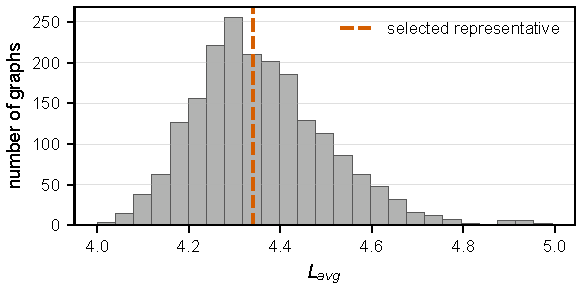
\includegraphics[width=\linewidth]{figures/Task_B_Strict_Layout_Fixed_test_p_0_ENG15_edited_part1}}
    \caption{Statistical distribution of the average shortest path length ($L_{avg}$) used to select a representative network topology at a fixed $p=0.15$. The horizontal axis represents the topological metric $L_{avg}$, the vertical axis displays the frequency of occurrences across an ensemble of randomly generated graph realizations ($N_{\mathrm{ens}} = 2000$). The red dashed vertical line marks the median of the distribution. Selecting the network realization closest to this median ensures that the subsequent spatial excitability analysis (Fig.~\ref{fig:excib_maps_represent}) is performed on a typical architecture, thereby avoiding statistically anomalous configurations.}
    \label{fig:lavg_selection}
\end{figure}
\begin{figure}[H]
    \centerline{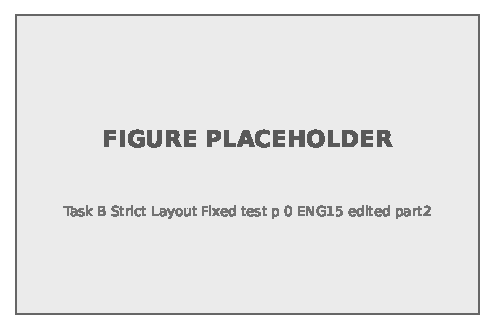
\includegraphics[width=\linewidth]{figures/Task_B_Strict_Layout_Fixed_test_p_0_ENG15_edited_part2}}
    \caption{Spatial maps of local excitability $B(k, i)$ (Eq.~\ref{eq:B_k_i}) for the first three non-trivial relaxation modes ($k=1, 2, 3$) on a rewired $10 \times 10$ lattice ($p = 0.15$). Each lattice node represents a waveguide site. All three panels share a common color scale to enable direct quantitative comparison across modes: bright (yellow/green) nodes strongly couple to the respective mode upon local single-photon injection, whereas dark (purple/black) nodes are effectively decoupled from the mode.}
    \label{fig:excib_maps_represent}
\end{figure}




\section{Heuristic Algorithm for Generating Initial States with a Pronounced Mpemba Effect}

As established in the previous section, topological disorder can induce a pronounced population-sector localization of the slowest relaxation mode ($k=1$). For the selected network, the independently calculated excitability map $B(1,i)$ exhibits a small bright region and an extended dark background. This mode-resolved spatial contrast makes it possible to construct initial states with tailored relaxation rates using a spectrally informed spatial approach.

In this section, we propose a deterministic heuristic algorithm that leverages the local excitability map $B(1,i)$ to construct a pair of diagonal (incoherent) initial density matrices exhibiting a pronounced Quantum Mpemba Effect. \textcolor{dark-green}{We present this algorithm as a proof-of-concept demonstration.} Rather than seeking the exact mathematical cancellation of the slowest mode projection ($c_1 \equiv 0$, which defines the strict 'Strong Mpemba' condition), our objective is to engineer a robust, \textcolor{dark-green}{physically observable and statistically exceptional} effect. For illustrative purposes and computational efficiency in extensive ensemble benchmarks, all algorithmic steps and benchmarks are presented for a selected representative $6 \times 6$ network at a rewiring probability $p=0.15$; the linear dimension of the Liouvillian matrix scales as $N^2$.

To examine the Mpemba effect, we refer to the state that is initially further from equilibrium as 'hot', since it relaxes more quickly, and to the state that is initially closer to equilibrium but relaxes more slowly as 'cold'.

\subsection{Step 1: Spectral analysis}
\begin{figure}[H]
    \centering
    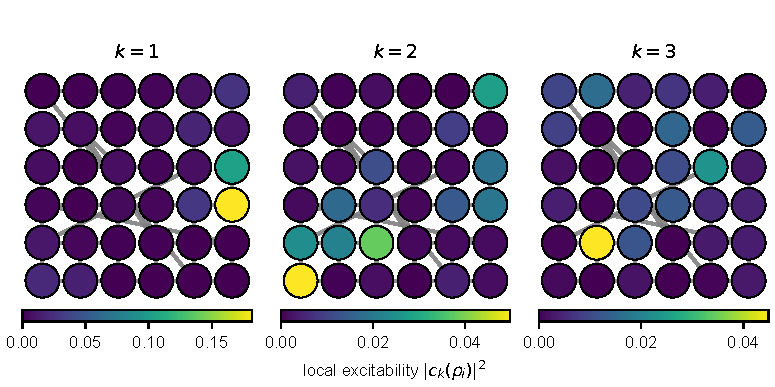
\includegraphics[width=0.9\linewidth]{figures/Step1_Three_Modes}
    \caption{Spatial maps of local excitability $B(k, i)$ for the first three non-trivial relaxation modes on the selected $6 \times 6$ test lattice ($p = 0.15$). The color mapping and node representation conventions strictly follow those detailed in Fig.~\ref{fig:excib_maps_represent}. All three modes exhibit spatially nonuniform excitability profiles; the state-engineering algorithm uses only the directly calculated contrast of the fundamental-mode map $B(1,i)$.}
    \label{fig:step1}
\end{figure}
The foundation of our algorithm is the spatial inhomogeneity of the system's response to local injection. As derived in Eq.~(\ref{local_excitability}), the excitability metric $B(k,i)$ translates the abstract bi-orthogonal eigenvectors into a physical map, revealing how strongly a single photon injected at site $i$ will excite the $k$-th relaxation channel.

Figure~\ref{fig:step1} illustrates these spatial excitability profiles. All three modes exhibit mode-dependent spatial concentration. For the fundamental mode ($k=1$), a small set of strongly coupled bright sites is separated from a broad background of weakly coupled dark sites. Our state-engineering protocol relies exclusively on this directly calculated excitability map.

\subsection{Step 2: Selection hot state (Dark node)}
To construct the 'hot' state, we find the darkest node on the map (the node that the least excites the first, slowest mode) and inject a photon into this node. The density matrix of the 'hot' state is a matrix with a single unit on the diagonal and all other elements equal to zero.

\subsection{Step 3: Selection cold state (Mix of bright nodes)}

To construct the 'cold' state, we select an integer $M$ ($2 \le M \le n^2/2$) and build a phase-compatible set $S_M$ of $M$ bright nodes. Starting from the node with the largest $|c_1(j)|$, nodes are added greedily: at each step we choose the node that maximizes the modulus of the accumulated coefficient $|\sum_{j\in S_M}c_1(j)|$. The 'cold' state is then formed as an incoherent, equally weighted statistical mixture,
\begin{equation}
    \rho_{\mathrm{cold}}(S_M)=\frac{1}{M}\sum_{j\in S_M}|j\rangle\langle j|,
    \qquad
    c_1^{\mathrm{cold}}(S_M)=\frac{1}{M}\sum_{j\in S_M}c_1(j).
    \label{eq:cold_state_selection}
\end{equation}
Thus, the selection uses the complex coefficients themselves rather than only the individual intensities $B(1,j)=|c_1(j)|^2$ and explicitly accounts for destructive sign or phase cancellation.

To determine the optimal number of bright nodes $M$, we evaluate the candidate mixtures using a heuristic objective function:
\begin{equation}
    Score(S_M) = \abs{\frac{c_1^{\mathrm{cold}}(S_M)}{c_1^{\mathrm{hot}}}}^2\cdot\abs{D_{\mathrm{hot}}-D_{\mathrm{cold}}(S_M)}.
    \label{eq:heuristic_score}
\end{equation}
This scoring formula acts as a balance between two fundamental requirements for a macroscopic QME. The first multiplier (the ratio of squared projections) enforces the spectral condition: the 'cold' state must strongly excite the slowest relaxation channel, while the 'hot' state remains essentially 'dark' to it. The second multiplier acts as a crucial geometric regularizer. It ensures that the selected states start sufficiently far apart in the relative entropy metric space ($\Delta D(0) > 0$), preventing the algorithm from converging to trivially close states that would yield physically meaningless, instantaneous micro-crossings.

\begin{figure}[H]
\centerline{
\begin{subfigure}{0.45\linewidth}
    \centering
    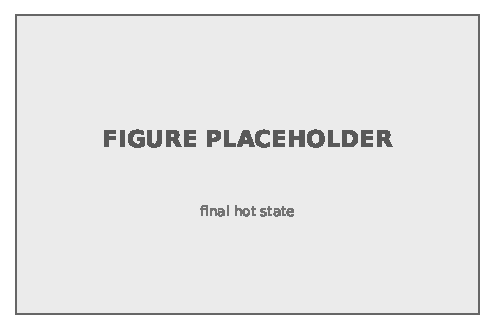
\includegraphics[width=0.8\linewidth]{figures/final_hot_state}
    \caption{"Hot" state (Darkest node)}
\end{subfigure}
\hfill
\begin{subfigure}{0.45\linewidth}
    \centering
    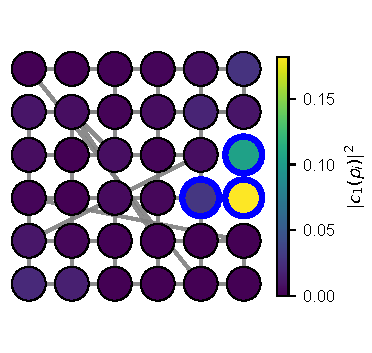
\includegraphics[width=0.8\linewidth]{figures/final_cold_state}
    \caption{"Cold" state ($M=3$ phase-compatible bright nodes)}
\end{subfigure}
}
\caption{Deterministic selection of the Mpemba pair based on the $k=1$ excitability map from Fig.~\ref{fig:step1}. \textbf{(A)} The localized "hot" state is placed at the darkest node (red outline), minimizing its interaction with the slow mode. \textbf{(B)} The mixed "cold" state is distributed across the phase-compatible set of $M=3$ bright nodes (blue outlines) selected by Eq.~(\ref{eq:cold_state_selection}); for this network the phase-aware rule retains the same three-node control state.}
\label{fig:step_hot_cold_selection}
\end{figure}

\subsection{Monte Carlo Benchmark and Applicability Limits}
\textcolor{dark-green}{Defining a universal, cross-system metric for the 'strength' of the QME remains a non-trivial challenge in open quantum systems, since absolute trajectory crossing times ($t^*$) are highly sensitive to the initial distance gap between states.} Since evaluating absolute optimality is hindered by this dependence, we assess the efficacy of the proposed deterministic algorithm by benchmarking it against a random Monte Carlo search within the fixed $6 \times 6$ network topology.

To ensure a physically meaningful comparison, we generated an ensemble of random pairs of diagonal density matrices whose population vectors were sampled from a uniform Dirichlet distribution, $\boldsymbol{\pi} \sim \mathrm{Dirichlet}(1, \dots, 1)$, ensuring unbiased coverage of the probability simplex. To discard trivial micro-crossings between states starting infinitesimally close, we applied a gap filter: the initial relative-entropy gap of a pair was required to be at least 10\% of the gap engineered by our algorithm, yielding an ensemble of $N_{\mathrm{adm}}=30\,000$ admissible pairs. For each pair, $D(t)$ was evaluated on $t\in[0,200]$ with step $\Delta t=0.5$, and the first crossing time $t^*$ was obtained by linear interpolation at the first sign change of $D_{\mathrm{cold}}(t)-D_{\mathrm{hot}}(t)$; unresolved crossings beyond $t=160$ were omitted.

\begin{figure}[H]
    \centering
    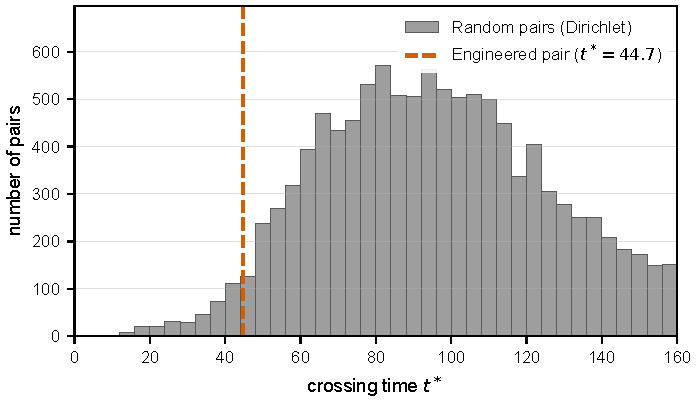
\includegraphics[width=0.9\linewidth]{figures/alg_compare}
    \caption{Statistical validation of the deterministic algorithm. The histogram shows the distribution of crossing times $t^*$ for an ensemble of $N_{\mathrm{adm}}=30\,000$ admissible random pairs (Dirichlet-sampled diagonal states) on the $6 \times 6$ network ($p=0.15$). The vertical dashed line marks the crossing time ($t^* = 44.7$) of the deterministically engineered pair from Fig.~\ref{fig:step_hot_cold_selection}: only $1.2\%$ of the admissible pairs cross faster. Crossings beyond $t \approx 160$, where both trajectories have relaxed to within the numerical resolution of equilibrium, are not physically resolved and are omitted.}
    \label{fig:algorithm_test}
\end{figure}

As illustrated in Fig.~\ref{fig:algorithm_test}, we find that the deterministically engineered pair significantly outperforms the random search: $N_{\mathrm{fast}}/N_{\mathrm{adm}}\approx1.2\%$ of the admissible random pairs achieve a faster crossing. To characterize the strength of the effect beyond the crossing time, we also evaluated, for the same ensemble, the maximal subsequent advantage $\Delta D_{\max} \equiv \max_t\,[D_{\mathrm{cold}}(t) - D_{\mathrm{hot}}(t)]$. The engineered pair crosses late in the relaxation, at $D(t^*) \approx 3.6\times10^{-3}$, and reaches $\Delta D_{\max} \approx 2.4\times10^{-4}$; these absolute values are necessarily small, since by the crossing time both trajectories are already close to equilibrium. Relative to the ensemble, however, the advantage is exceptional: only $0.14\%$ of the admissible random pairs achieve a larger $\Delta D_{\max}$ (the 99.86th percentile), while the median ensemble advantage lies at the numerical noise floor ($\sim 10^{-15}$), i.e., a typical admissible pair never overtakes at all.

\textcolor{dark-green}{Finally, we note the physical limits of applicability for the proposed proof-of-concept heuristic. The current algorithm relies exclusively on the spatial excitability structure of the single fundamental mode $v_1$. Consequently, its validity is contingent upon the network possessing a strongly concentrated fundamental-mode excitability profile and a distinct eigenvalue gap separating this mode from the rest of the spectrum. In arbitrary random ensembles, topological fluctuations can lead to quasi-degeneracies ($\lambda_1 \approx \lambda_2$) or delocalization of the fundamental-mode excitability, which would necessitate accounting for higher-order relaxation channels. The generalization of this mode-resolved spatial approach to multi-mode heuristics across broad topological ensembles remains a subject for future investigation.}
% \section{Future Work}

% \begin{itemize}
%     \item Explain the absence of a complex component in the newly emerging modes.
%     \item Measure larger networks to verify the persistence of the effects.
%     \item Investigate symmetric modes more closely, specifically the differences between even and odd lattices.
%     \item Analyze more than the first three modes and visualize the data to clearly track the emergence of the "topological effect".
%     \item Construct physical states for the new effect and identify the Mpemba effect.
%     \item Implement more complex rewiring models.
%     \item Perform analysis via diagram superposition.
% \end{itemize}


\section{Conclusion}

We have presented a systematic study of the Quantum Mpemba effect
in networks of coupled optical waveguides, progressing from regular
square lattices to topologically disordered graphs.

For regular lattices, we find from the spectral decomposition of the
Liouvillian superoperator that the relaxation eigenmodes possess
well-defined macroscopic geometric patterns dictated by lattice
symmetries. Exploiting this spatial regularity, we constructed a set
of candidate initial states with highly selective mode content and
confirmed that specific pairs of these states exhibit trajectory
crossings in the relative-entropy distance to equilibrium---the
hallmark of the Mpemba effect. The effect was observed robustly for
square lattices of sizes $n = 5$ through $n = 11$.

Introducing topological disorder via a Watts--Strogatz-type
edge-rewiring procedure, we track the evolution of the relaxation
spectrum across the lattice-to-random crossover. We establish three
key findings. First, the relaxation rate of the slowest mode
$\mathrm{Re}\,\lambda_1$ \rev{is non-monotonic in the rewiring
probability: its magnitude first grows, peaking near $p \approx 0.03$,
and then decreases toward the random-graph limit}, indicating that certain disordered configurations
host anomalously slow relaxation channels---a spectral phenomenon we identify as topology-induced population-sector localization of the slow mode. Second, the Inverse Participation
Ratio and the community-overlap analysis demonstrate that the diagonal component of the slowest
mode becomes strongly concentrated within a small subset of network nodes. The corresponding
components of the second and third modes also localize, but more weakly. Third, the directly
calculated local-excitability map of the fundamental mode exhibits a pronounced contrast between
bright and dark sites, providing a spectrally informed spatial route to engineering initial states with
suppressed overlap with the slowest relaxation channel.

Building on these observations, we formulated a deterministic
heuristic algorithm for constructing pairs of initial diagonal density
matrices that maximize the Mpemba effect on a given disordered
network. The algorithm places the ``hot'' (far-from-equilibrium,
fast-relaxing) state at the node with the smallest local excitability
for the first mode, and distributes the ``cold''
(closer-to-equilibrium, slow-relaxing) state across a phase-compatible
set of $M$ bright nodes selected from the complex projection coefficients,
with $M$ optimized via a scoring function that balances the
projection ratio and the initial distance gap. A benchmark against
$30\,000$ admissible random diagonal-state pairs on a $6 \times 6$
lattice at $p = 0.15$ confirmed that only about $1.2\%$ of them
achieve a faster crossing than the algorithmically engineered pair,
validating the approach as a proof of concept.

Several directions for future work merit attention.
The present analysis is restricted to incoherent (diagonal) initial
states; extending the algorithm to coherent superpositions may
further amplify the effect by exploiting off-diagonal interference.
Likewise, incorporating site-resolved photon losses (beyond the
uniform attenuation that factors out of the normalized dynamics)
would bring the model closer to realistic photonic hardware.
Scaling the approach to larger networks ($n \gg 10$) will require
efficient spectral methods or variational approximations, since, for a
graph of $N$ nodes, the Liouvillian acts on the $N^2$-dimensional space
of density matrices and is represented by an $N^2 \times N^2$ matrix,
whose dense storage scales as~$N^4$.  It would also be valuable to
investigate alternative graph families---such as scale-free,
hierarchical, or empirical real-world networks---to assess the universality of the topology-induced population-sector mode localization.  Finally,
the connection between the topologically assisted Quantum Mpemba effect and Liouvillian exceptional points, recently highlighted in the context
of trapped-ion experiments~\cite{Zhang2025}, deserves further theoretical
exploration in the network setting.  From an experimental
perspective, the model maps directly onto photonic mesh lattices with
controllable dephasing~\cite{Longhi2024,Longhi2024bosonic}, suggesting that the predicted effects
are within reach of current integrated-photonic and fiber-loop
platforms.

\backmatter

\bmhead{Acknowledgements}
The work was financially supported by [Prioritet 2030] (project No. ...).


\section*{Data availability}

The code and data used for the numerical simulations and figure generation in this study are available on GitHub at \url{https://github.com/alpha7en/mpemba_quantum_effect}.

\section*{Declarations}
\textbf{Conflict of interest.} The authors declare no conflict of interest.

\bibliography{refs}

\end{document}